\begin{figure}[H]
  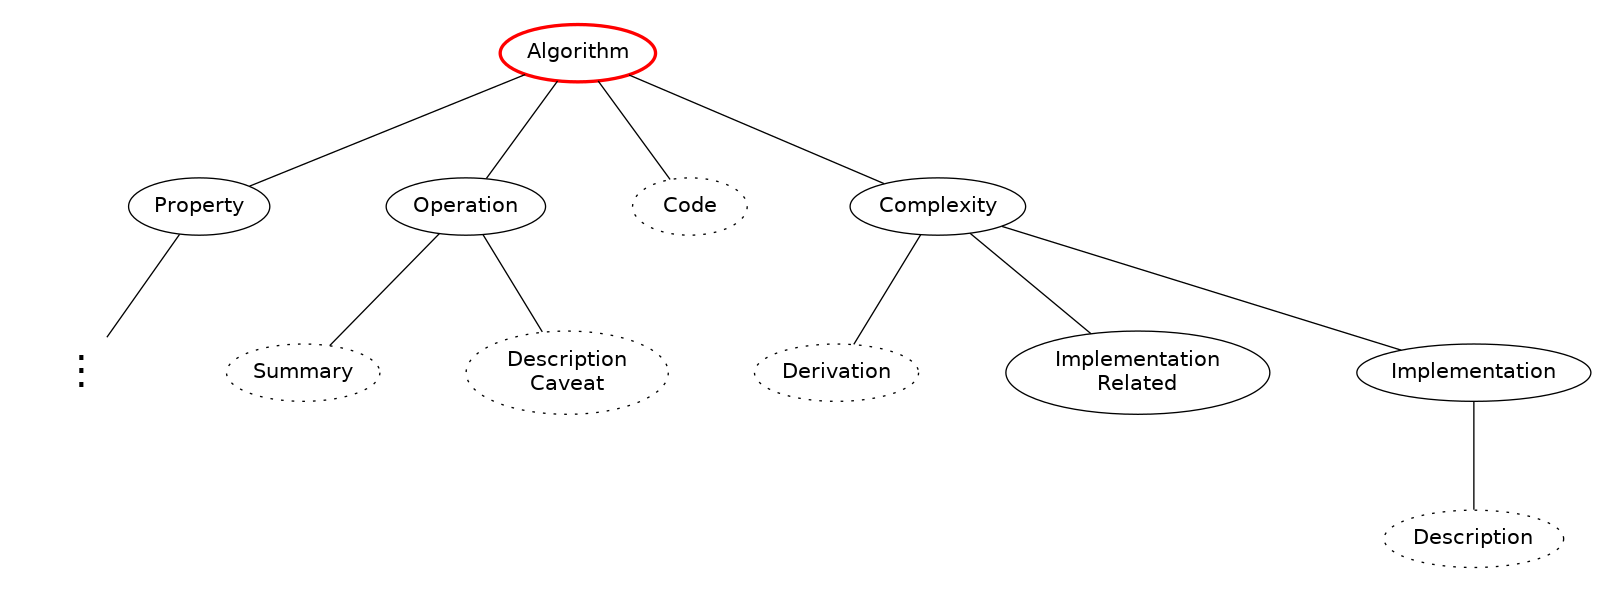
\includegraphics[scale=0.2]{DJK_tree}
  % \begin{tikzpicture}
  %   [
  %   grow                    = right,
  %   node distance           = 7em,
  %   edge from parent/.style = {draw, -latex},
  %   every node/.style       = {font=\footnotesize},
  %   sloped
  %   ]
  %   \node [root] (0) {Algorithm};
  %   \node [env] (1) [below left of=0] {History};
  %   \node [leaf] (1) [below left of=0] {History};
  %   \node [env] (2) [right of=1] {Problem};
  %   \node [env] (3) [right of=2] {Operation};
  %   \node [env] (4) [right of=3] {Complexity};
  %   \node [env] (5) [below left of=3] {Implementation};
  %   \node [env] (6) [below right of=4] {Implementation};
  %   \node [leaf] (7) [below right of=4] {Implementation};
    
  %   \path [-]
  %   (0) edge (1)
  %   (0) edge (2)
  %   (0) edge (3)
  %   (0) edge (4)
  %   (4) edge (5)
  %   (4) edge (6)
  %   (1) edge [below, out=290, in=260, looseness=8, distance=1.6cm]
  %   node [swap] {Assumption} (1);
    
  % \end{tikzpicture}
\todo{Fix this caption, How to show an edge that leads to unshown subtrees?}
\caption{Explanation Tree for Dijkstra's 004}
\label{fig:djk-tree}
\end{figure}